\documentclass[a4paper,11pt,spanish]{article}

\textwidth 18.5cm
\textheight 26cm
\topmargin -2cm
\oddsidemargin -1.5cm
\parskip .3em
\parindent 0cm
\pagestyle{empty}

%your favourite packages here
\usepackage[spanish]{babel}
% \usepackage{lineno}
% \usepackage{mathptmx}
%\usepackage{psfrag,graphicx}
\usepackage{amsmath} 
\usepackage{amssymb} 
\usepackage{amsfonts}
\usepackage{bm}
%\usepackage{bbm}
\usepackage{color}
\usepackage{latexsym}
\usepackage{epstopdf}
\usepackage{color}
%\usepackage{times}

\usepackage{psfrag,graphicx} 
%\usepackage{picins} 
\usepackage{natbib}
\usepackage{epstopdf}\DeclareGraphicsRule{.tif}{png}{.png}{`convert #1 `basename
#1 .tif`.png}
%\usepackage{dsfont}
%\usepackage{mathtools}

\definecolor{mygrey}{gray}{0.35}
\definecolor{myblue}{rgb}{0.2,0.2,0.8}
\definecolor{myzard}{cmyk}{0,0,0.05,0}
\definecolor{mywhite}{rgb}{1,1,1}
\definecolor{myred}{rgb}{1,0.,0.3}

\def \barl {\begin{array}{rl}} 
\def \ea {\end{array}}
%\definecolor{myblue}{named}{MidnightBlue}
\usepackage[colorlinks=true,citecolor=myblue,linkcolor=myred]{hyperref}
\def\beq{\begin{equation}}
\def\eeq{\end{equation}}
\def\ba{\begin{align}}
\def\enda{\end{align}}
\def\bi{\begin{itemize}}
\def\ei{\end{itemize}}
\def\bs#1{\boldsymbol{#1}}
\def\txt#1{\textrm{#1}}

\newcommand{\eq}[1]{Eq.\;(\ref{#1})}

\newcommand{\sgn}{\operatorname{sgn}}
\def\C{{\mathbb{C}}} \def\F{{\mathbb{F}}}
\def\N{{\mathbb{N}}} \def\Q{{\mathbb{Q}}}
\def\R{{\mathbb{R}}} \def\Z{{\mathbb{Z}}}
\def\cH{{\mathcal H}}
\def\bfsigma{\boldsymbol{\sigma}}
\def\bfmu{\boldsymbol{\mu}}
\def\dd{\mathord{\rm d}} \def\Det{\mathop{\rm Det}}
\def\dist{\mathop{\rm dist}} \def\ee{\mathord{\rm e}}
\def\End{\mathord{\rm End}} \def\ev{\mathord{\rm ev}}
\def\id{\mathord{\rm id}} \def\ii{\mathord{\rm i}}
\def\min{\mathord{\rm min}} \def\mod{\mathord{\rm mod}}
\def\prob{\mathord{\rm prob}}
\def\tr{\mathop{\rm Tr}}
\def\half{\textstyle\frac{1}{2}}
\def\third{\textstyle\frac{1}{3}}
\def\fourth{\textstyle\frac{1}{4}}

\graphicspath{{figs/}}

\newcommand{\da}{\downarrow}
\newcommand{\ua}{\uparrow}

\renewcommand{\ii}{{\rm i}}
\renewcommand{\ee}{{\rm e}}

%brackets
 \newcommand{\ket}[1]{|#1\rangle}
 \newcommand{\bra}[1]{\langle #1|}
 \newcommand{\braket}[2]{\langle #1|#2\rangle}

 \newcommand{\ketbra}[2]{\ket{#1}\bra{#2}}
 \newcommand{\proj}[1]{\ketbra {#1}{#1}}
 \newcommand{\biket}[2]{\ket{#1\;#2}}
 \newcommand{\bibra}[2]{\bra{#1\;#2}}
 %\newcommand{\ketbradif}[2]{\biket {#1}{#2}\bibra {#1}{#2}}
 \newcommand{\preespacio}{\!\text{\hspace{0.2 ex}}}
 \newcommand{\postespacio}{\!\text{\hspace{0.75 ex}}}


% \graphicspath{{Plots/}}

\begin{document}

%\title[Short Title]{Ejercicios para el curso de Introducci\'on a la \'Optica Cu\'antica}

\author{C. Cormick}

% \maketitle

\noindent{\large \bf Repaso 1ra parte - Procesamiento Cu\'antico de la Informaci\'on - FING, 1er semestre 2025}


\bigskip

\begin{enumerate}
 \item Supongamos que tenemos un estado de dos qubits de la forma: \vspace{-5pt}

 \begin{center}
  
\includegraphics[width=120pt]{repaso_2qubits.png}
 \end{center}
 \vspace{-5pt}

 donde $a, b, c \in \mathbb{C}$.

 \begin{enumerate}
  \item Escribir qu\'e condici\'on deben cumplir $a,b,c$ para que el estado est\'e normalizado. En lo sucesivo suponer que esa condici\'on se cumple.
  \item Calcular la probabilidad de cada resultado si se miden los dos qubits.
  \item Calcular ahora la probabilidad de cada resultado si se mide solamente el primer qubit.
  \item Suponer que se realiza la medici\'on sobre el primer qubit \'unicamente. Indicar cu\'al es el estado posterior a la medici\'on en cada caso, escribiendo dicho estado en forma normalizada.
\end{enumerate}

\vspace{10pt}

\item Mostrar que las matrices $I, X, Y, Z$ son una base para todas las matrices de $2\times2$ (con coeficientes
complejos), es decir que toda matriz de este tipo puede escribirse como combinación lineal de $I, X, Y, Z$.

\vspace{10pt}

\item Consideramos el c\'odigo contra bit-flips en una versi\'on ``comprimida'' como se muestra en la figura:
    
    \begin{center}
     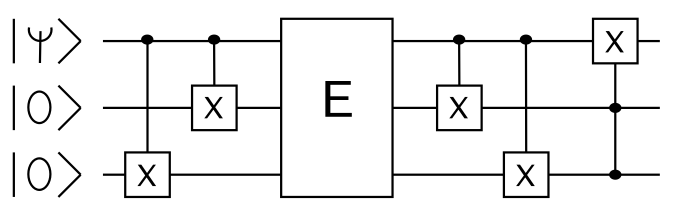
\includegraphics[width=200pt]{bit-flip.png}
    \end{center}

    En esta figura, $\ket{\psi} = a\ket{0} + b\ket{1}$ es un estado arbitrario desconocido de un qubit, y la caja $E$ representa un posible canal ruidoso. En esta versi\'on del c\'odigo, en lugar de la medici\'on de la paridad a trav\'es de qubits auxiliares y la posterior correcci\'on de los errores dependiendo de los resultados obtenidos, la correcci\'on se implementa a trav\'es de las compuertas que aparecen luego del posible error (la \'ultima compuerta es la de Toffoli).
    
    \begin{enumerate}
     \item Mostrar que, si $E$ corresponde a la aplicaci\'on de la identidad o de una compuerta $X$ sobre uno (solo uno, pero cualquiera) de los tres qubits, entonces en el final del circuito el primer qubit (el de arriba) vuelve a su estado original $\ket{\psi}$, y queda desentrelazado de los qubits auxiliares.
     \item Mostrar que midiendo el estado final de los qubits auxiliares se puede averiguar cu\'al fue el error que ocurri\'o (suponiendo que $E$ es una de las cuatro opciones: $I$, $X_j$ con $j=1,2,3$).
     \item Mostrar a trav\'es de un ejemplo que si el error $E$ no es de la forma del \'item anterior entonces no siempre puede corregirse.
    \end{enumerate}

\end{enumerate}

\end{document}
